\ctitle{Enzymer}

\paragraph{Dette kapittelet} forklarer hva proteiner er laget av og hvordan de er bygd opp. Så går vi nærmere på enzymer og hvordan de fungerer. Mot slutten også noen eksempler på enzymer, enzymkatalyserte reaksjoner og bioteknologiske løsninger som tar i bruk enzymer.

\cstitle{Proteiner} \index{proteiner}

\paragraph{Aminosyrer}\index{aminosyrer} Karbon bundet til et hydrogenatom, en karboksylsyregruppe og en aminogruppe, samt en såkalt R-gruppe som kan være mye rart (upolar alifatisk som i glysin, aromatisk som i fenylalanin, polar uladd som i serin, positivt ladd som i lysin, negativt ladd som i aspartat). 9 av de 20 aminosyrene som brukes i proteinsyntese er \ix{essensielle aminosyrer} som må opptas gjennom mat. 

\paragraph{\ix{D- og L-stereoisomeri}} En type \ix{stereoisomeri} for aminosyrer, som fungerer som følger: hvis man lar hydrogenatomet gå inn i arket, har man L-formen hvis gruppene som går mot klokka er \ce{COOH -> R -> NH_2}, og D-formen hvis man får denne rekkefølgen ved å gå med klokka.
\begin{center}
	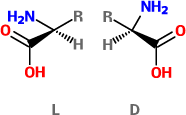
\includegraphics[scale=0.5]{enantiomers.png}
\end{center}
Av en eller annen grunn finnes kun L-enantiomerene til aminosyrene i proteiner. D-aminosyrer finnes andre steder i naturen, der de fungerer som mellomtrinn i aminosyremetabolisme, i polypeptider i celleveggene til noen bakterier, og som nevrotransmittere (signalstoffer). Det har også blitt syntetisert proteiner av D-enantiomerer i laboratoriet - disse vil være speilbilder av proteinene som dannes fra L-enantiomerene.

\paragraph{Peptidbinding} Aminosyrer bindes sammen via peptidbindinger i lange polymerer som vi kaller proteiner. En \ix{peptidbinding} dannes gjennom en kondensasjonsreaksjon når \ce{H} fra en aminogruppe og \ce{OH} fra en karboksylsyregruppe går ut som et vannmolekyl, og legger igjen en binding som ser slik ut:
\begin{center}
	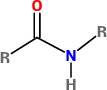
\includegraphics[scale=0.5]{peptide}
\end{center}
På grunn av \ix{resonans} i peptidbindingen (i resonansstrukturen som ikke er vist i figuren, blir \ce{C=O}-bindingen til en \ce{C-O^-}-binding, mens \ce{C-N}-bindingen blir til en \ce{C=N^+}-binding) kan ikke molekylet rotere rundt en peptidbinding, og alle atomene som inngår i en peptidbinding (C, O, N, H) ligger i samme plan.

\paragraph{Peptider} Korte kjeder av aminosyrer kalles \ix{peptider} og navngis ved å begynne på den terminale aminogruppen, traversere peptidet til man støter på den terminale karboksylsyregruppen, og ramse opp alle aminosyrene på veien. Fullstendig navngivning av proteiner er dermed upraktisk, men det som er så fint er at det finnes altså en russisk fyr som har uttalt hele det fullstendige systematiske navnet til verdens lengste protein (\ix{titin}). Det tok så lang tid at man kunne se forskjellen i skjeggvekst på starten og slutten av opptaket.

\paragraph{Primærstrukturen til proteiner}\index{primærstruktur} er sekvensen av aminosyrer, samt eventuelle disulfidbindinger mellom cysteingrupper. Primærstrukturen gir opphav til sekundær- og tertiærstruktur (men du blir ikke akkurat så mye klokere på høyere ordens struktur ved å se på aminosyresekvensen). 

\paragraph{Sekundærstrukturen til proteiner}\index{sekundærstruktur} er lokale strukturer i proteinet. Det er bare to slike strukturer vi snakker noe særlig om: $\alpha$-helikser og $\beta$-flak.

\paragraph{\ix{$\alpha$-heliks}} Proteinet kan kveile seg i en spiral, som kan være venstre- eller høyrehendt. Denne strukturen stabiliseres av hydrogenbindinger langs spiralens akse. I en slik spiral kan man for eksempel ha at en side er hydrofob, mens den andre er hydrofil.

\paragraph{\ix{$\beta$-flak}} Flak som dannes når rette ``tråder'' av proteinet bretter seg frem og tilbake, med hydrogenbindinger mellom trådene. Hvis trådene går i samme retning, er flaket parallelt, og hvis de går i alternerende retninger er flaket antiparallelt. $\beta$-flak er foldet i ``trekkspill-mønster'', og R-gruppene på aminosyrene vil stå ut av flaket.

\paragraph{Tertiærstrukturen til proteiner}\index{tertiærstruktur} er den tredimensjonale strukturen som reflekterer proteinets funksjon. Slik struktur er stabilisert av hydrofobe interaksjoner med vann (hydrofobiske grupper vender seg mot midten av proteinet og hydrofile grupper vender seg utover) samt hydrogenbindinger og ioniske interaksjoner som optimaliseres i de mest termodynamisk stabile strukturene. Disse interaksjonene gjør at proteiner har en tendens til å ``krølle seg sammen'' til den karakteristiske klumpete formen.

\paragraph{Kvartærstrukturen til proteiner}\index{kvartærstruktur} I noen tilfeller er det flere proteiner, eller flere molekyler av det samme proteinet, som går sammen for å danne en større struktur. Denne strukturen kalles da kvartærstrukturen til proteinet. Et eksempel på et protein med kvartærstruktur er \ix{hemoglobin}, der 4 polypeptidkjeder går sammen for å danne én funksjonell enhet.

\cstitle{Enzymer}

\paragraph{Enzym}\index{enzym} Biologisk katalysator som får reaksjonene i cellen til å gå raskere ved å senke aktiveringsenergien til reaksjonene.

\paragraph{Struktur til enzymer} De fleste enzymer er proteiner. Det finnes også enzymer som består helt eller delvis av RNA, disse kalles \ix{ribozym}er. Proteiner er bygget opp av aminosyrer som er kovalent bundet til hverandre i lange kjeder. Et område på en enzym der det foregår en reaksjon kalles et \idx{aktivt sete}.

\paragraph{Substrat} Enzymer er gjerne veldig spesifikke, i så stor grad at proteinet har en fysisk form der molekylet som skal prosesseres (dette molekylet kalles \idx{substrat}et) passer inn. 

\paragraph{Nøkkel-i-lås}\index{nøkkel-i-lås} Dette var den første hypotesen om samspillet mellom enzymet og substratet: at substratet passer perfekt inn i enzymet fordi enzymet er en romlig negativ av substratet. En slik hypotese forklarer hvordan enzymer kan være så spesifikke.

\paragraph{Hånd-i-hanske}\index{hånd-i-handske} Det har vist seg at substratet fungerer mer som en hånd i en handske, fordi substratet og enzymet kan påvirke hverandre underveis i reaksjonen. Enzymet og substratet er altså litt mer fysisk fleksible enn nøkkel-i-lås-analogien skulle tilsi.

\paragraph{Lysozym}\index{lysozym} er det første proteinet som ble analysert ned til den minste atomære detalj. Lysozym hydrolyserer bindingen mellom sukkerring 4 og 5 i et molekyl som består av 6 sukkerringer. 

\paragraph{Glukoseoksidase} Dette proteinet omformer $\beta-D$-glukose, men ingen andre sukkerarter eller karbohydrater, til glukonolaton. Dette er fordi det kun er $\beta-D$-glukose som er lite nok og passer akkurat inn i den romlige strukturen til \ix{glukoseoksidase}. Glukoseoksidase er med andre ord svært \ix{substratspesifikt enzym}.

\paragraph{Mulige årsaker til \ix{reduksjon i aktiveringsenergi}} Enzymer kan redusere aktiveringsenergien til en reaksjon. Enzymet binder seg ikke til substratet i sin opprinnelige konfigurasjon, men til en mellomtilstand som kan være deformert i forhold til det originale stoffet.

Inne i enzymet er svært reaktive funksjonelle grupper konsentrert på et veldig lite område, og satt sammen på en måte som gjør at de er i direkte kontakt med bindingene i substratet som skal modifiseres. Området rundt det aktive setet består stort sett av upolare grupper, som gjør at enzymet lokalt ligner på en organisk (upolar) løsning. Dermed blir de få polare gruppene i nærheten svært reaktive i forhold til det de ville vært i vandig løsning.

\paragraph{Kofaktorer}\index{kofaktor} Kjemiske stoffer som ikke er proteiner, og som et enzym krever for å utføre oppgaven sin. Typisk inorganiske molekyler som \ce{Fe^3+}, \ce{Mg^2+}, \ce{Mn^2+} og \ce{Zn^2+}.

\paragraph{Koenzymer}\index{koenzym} Organiske forbindelser som binder seg til eller i nærheten av det aktive setet. De modifiserer strukturen til substratet eller beveger elektroner, protoner eller kjemiske grupper mellom substratet og enzymet. I motsetning til enzymene selv brukes koenzymer opp i enzymkatalyserte reaksjoner. Mange av disse kommer fra vitaminer, for eksempel NAD$^+$ fra vitamin B.

\paragraph{Klassifisering av enzymer} Det finnes seks typer enzymer, som navngis etter hva de gjør:
\begin{itemize}[nolistsep,noitemsep]
	\item \idx{oksidoreduktaser} reduserer ett stoff og oksiderer et annet,
	\item \idx{transferaser} overfører kjemiske grupper fra et stoff til et annet (gjerne ved hjelp av koenzymer),
	\item \idx{hydrolase}r kløyver stoffer med addisjon av vann,
	\item \idx{lyaser} kløyver stoffer uten addisjon av vann (og danner gjerne dobbeltbindinger eller ringstrukturer),
	\item \idx{isomeraser} omdanner et molekyl til en annen isomer, og 
	\item \idx{ligaser} bruker ATP for å binde sammen to stoffer.
\end{itemize}

\paragraph{Eksempler på enzymer og \ix{enzymkatalyserte reaksjoner}}
\begin{itemize}[noitemsep,nolistsep]
	\item \emph{Ekstracellulære hydrolaser}\index{hydrolase} produseres av mikrober og slippes ut i miljøet for å degraderer biopolymerer til mindre enheter som kan tas opp av mikroben. De brukes også av edderkopper til såkalt ekstraintestinal fordøyelse. Ekstracellulære hydrolaser er av naturlige grunner de enzymene som er enklest og billigst å ekstrahere fra en cellekultur - det er ikke noen cellemembran mellom deg og enzymet. De fire neste eksemplene er \ix{ekstracellulære hydrolaser}.
	\item Malt inneholder \idx{amylaser}, som bryter opp stivelse til kortere oligosakkarider, samt glucoamylase, som bryter opp oligosakkarider til glukose. Disse enzymene kan brukes i baking for å bryte ned stivelse til sukker og dermed akselerere heving, samt for å degradere klebrig gluten og gjøre deigen luftigere. I tekstilindustrien tilsetter man gjerne stivelse for å få fibrene til å holde seg sammen under veving. Amylaser brukes til å fjerne stivelse når vevingen er ferdig.
	\item \emph{Pektinaser}\index{pektinase} bryter ned de store pektinmolekylene i frukt for å gjøre juicen mindre tyktflytende. Hvis man ikke fjerner pektin, får juicen en gel-aktig konsistens som er uønsket og vanskelig å håndtere. Pektinaser hentes fra \idx{Aspergillus}- og \idx{Rhizopus}-sopp.
	\item Papaya, fiken og ananas inneholder \idx{proteaser} som bryter ned bindevev i kjøtt, og dermed gjør det mørere. De samme enzymene brukes også for å mykne lær. 
	\item \emph{Hydrolaser med lav substratspesifisitet}: brukes som vaskemidler som bryter ned fett og proteiner, som binder seg til fibrene i tøy. Fett og proteiner er ``limet'' som gjør at skitt setter seg fast i klær. Enzymer er nyttige fordi de gjør at man kan gjøre oppvasken på relativt lav temperatur. Før i tida måtte slike enzymer hentes ut fra bukspyttkjertler til dyr, men etter at enzymet \ix{subtilisin} ble oppdaget i \idx{Bacillus licheniformis}  på 60-tallet, inneholder vaskemiddel som regel hydrolytiske enzymer fra mikroorganismer. Andre enzymer som brukes i vaskemiddel er cellulaser, som bryter ned mikrofibre i bomull og gjør stoffet mer mykt, og amylaser og lipaser som fjerner matrester i vaskemaskiner.
	\item Fosfor i planter lagres gjerne i form av fytat, en seksringet forbindelse. Mennesker og dyr klarer ikke å ta opp fosfor i denne formen, men det finnes mikrobiell \idx{fytase} som hydrolytisk kløyver fytat slik at man ender opp med fosfat, som vi kan ta opp. Fytaser er et spesielt nyttig tilskudd i grisefôr, fordi man slipper å tilsette så mye miljøskadelig fosfat (kapittel 6) i fôret.
	\item \emph{Glukoseisomerase}\index{glukoseisomerase}: brukes til å omdanne glukose til fruktose, som er søtere enn glukose (og sukrose). 
\end{itemize}

\paragraph{Immobiliserte enzymer}\index{immobilisering} Enzymer som på en eller annen måte sitter fast i et medium. Metoder for å immobilisere enzymer inkluderer adsorbsjon til fibre, kovalente bindinger til fibre, krysslinking mellom enzymer, immobilisering i gel eller hule fibre og mikrokapsler. 

Det som er fint med immobiliserte enzymer, er at de kan utføre reaksjoner under kontrollerte betingelser uten å legge igjen enzymrester i produktet (nyttig for å forhindre immunreaksjoner i pasienter). Samtidig blir mindre av enzymet kastet bort; enzymet er resirkulerbart. 

\paragraph{Enzymkilder}\index{enzymkilder} Hvis vi vil ha tak i enzymer til eget bruk, har vi forskjellige kilder. Av det som ikke er nevnt tidligere: Bukspyttkjertler, spesielt til gris, inneholder mye fint: trypsin, chymotrypsin, lipaser og amylaser. Magesekker inneholder pepsin. En av de nyttigste enzymkildene er mikroorganismer, som er veldig greie å ha med å gjøre og kan gros på laben og i reaktorer - og via genteknologi kan enzymene skreddersys. Det finnes også mange bruksområder for enzymene som dannes av ekstremofile mikroorganismer, for eksempel DNA polymerase, som vi skal se blir nyttig i analytisk bioteknologi (kapittel 10).